\section{Color\-Image\-Data Class Reference}
\label{class_c_s_image_viewer_1_1_color_image_data}\index{CSImageViewer::ColorImageData@{CSImageViewer::ColorImageData}}
class containing the actual pixel data for a color image (3 values per pixel - red, green, and blue (rgb))  


Inheritance diagram for Color\-Image\-Data::\begin{figure}[H]
\begin{center}
\leavevmode
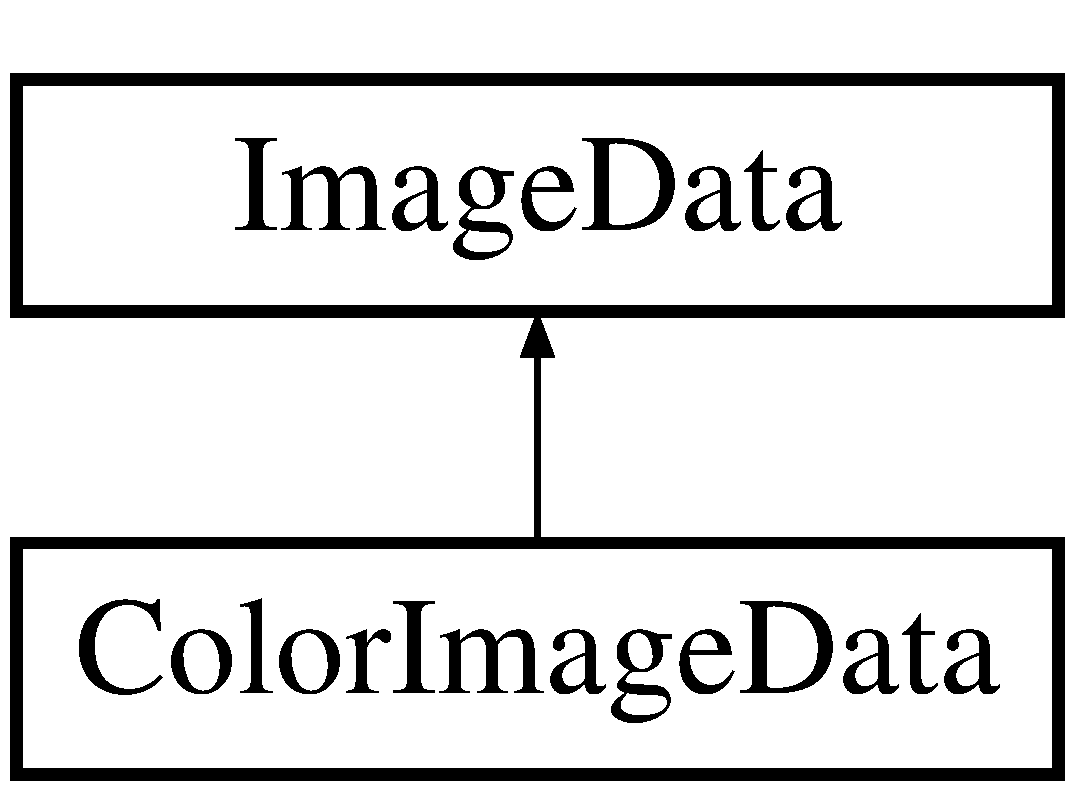
\includegraphics[height=2cm]{class_c_s_image_viewer_1_1_color_image_data}
\end{center}
\end{figure}
\subsection*{Public Member Functions}
\begin{CompactItemize}
\item 
{\bf Color\-Image\-Data} (Bitmap old\-BM)
\begin{CompactList}\small\item\em Given a bitmap image, this ctor reads the image data, stores the raw pixel data in an array, and creates a displayable version of the image. m\-Original\-Data will be allocated and set to the pixel values in the bitmap. \item\end{CompactList}\item 
{\bf Color\-Image\-Data} (Bitmap old\-BM, Color[$\,$] old\-Palette, int bpp)
\begin{CompactList}\small\item\em Given a bitmap image and a palette (i.e., color lookup table used to translate scalar image values into other color values), this ctor reads the image data, uses the lookup table to store the pixel data in an array, and creates a displayable version of the image. m\-Original\-Data will be allocated and set to the pixel values in the bitmap. \item\end{CompactList}\item 
{\bf Color\-Image\-Data} (int[$\,$] unpacked, int w, int h)
\begin{CompactList}\small\item\em This ctor constructs a {\bf Color\-Image\-Data}{\rm (p.\,\pageref{class_c_s_image_viewer_1_1_color_image_data})} object from an array of rgb pixel values and the width and height of the image. m\-Original\-Data will be allocated and set to the pixel values in unpacked. \item\end{CompactList}\item 
void {\bf unpacked\_\-rgb\_\-to\_\-display} (int[$\,$] unpacked)
\begin{CompactList}\small\item\em This function takes an unpacked int array of rgb pixel values (representing an entire image), and copies the values to m\-Display\-Data (also representing an entire image). m\-Display\-Image is changed to these values as well. m\-Original\-Data remains unchanged. Note that unpacked must be the same size as the original image (m\-W$\ast$m\-H). \item\end{CompactList}\item 
int {\bf get\-Red} (int row, int col)
\begin{CompactList}\small\item\em Given a pixel's row and column location, this function returns the value of the pixel's red component. \item\end{CompactList}\item 
int {\bf get\-Green} (int row, int col)
\begin{CompactList}\small\item\em Given a pixel's row and column location, this function returns the value of the pixel's green component. \item\end{CompactList}\item 
int {\bf get\-Blue} (int row, int col)
\begin{CompactList}\small\item\em Given a pixel's row and column location, this function returns the value of the pixel's blue component. \item\end{CompactList}\end{CompactItemize}


\subsection{Detailed Description}
class containing the actual pixel data for a color image (3 values per pixel - red, green, and blue (rgb)) 



\subsection{Constructor \& Destructor Documentation}
\index{CSImageViewer::ColorImageData@{CSImage\-Viewer::Color\-Image\-Data}!ColorImageData@{ColorImageData}}
\index{ColorImageData@{ColorImageData}!CSImageViewer::ColorImageData@{CSImage\-Viewer::Color\-Image\-Data}}
\subsubsection{\setlength{\rightskip}{0pt plus 5cm}{\bf Color\-Image\-Data} (Bitmap {\em old\-BM})}\label{class_c_s_image_viewer_1_1_color_image_data_f8056c730cb6b923376592834303e1b5}


Given a bitmap image, this ctor reads the image data, stores the raw pixel data in an array, and creates a displayable version of the image. m\-Original\-Data will be allocated and set to the pixel values in the bitmap. 

\begin{Desc}
\item[Parameters:]
\begin{description}
\item[{\em old\-BM}]bitmap image used to construct an instance of this class \end{description}
\end{Desc}
\begin{Desc}
\item[Returns:]nothing (ctor) \end{Desc}
\index{CSImageViewer::ColorImageData@{CSImage\-Viewer::Color\-Image\-Data}!ColorImageData@{ColorImageData}}
\index{ColorImageData@{ColorImageData}!CSImageViewer::ColorImageData@{CSImage\-Viewer::Color\-Image\-Data}}
\subsubsection{\setlength{\rightskip}{0pt plus 5cm}{\bf Color\-Image\-Data} (Bitmap {\em old\-BM}, Color[$\,$] {\em old\-Palette}, int {\em bpp})}\label{class_c_s_image_viewer_1_1_color_image_data_0221e86bc6947ba666b133666ed7bac6}


Given a bitmap image and a palette (i.e., color lookup table used to translate scalar image values into other color values), this ctor reads the image data, uses the lookup table to store the pixel data in an array, and creates a displayable version of the image. m\-Original\-Data will be allocated and set to the pixel values in the bitmap. 

\begin{Desc}
\item[Parameters:]
\begin{description}
\item[{\em old\-BM}]bitmap image used to construct an instance of this class \item[{\em old\-Palette}]color lookup table \item[{\em bpp}]bits-per-pixel \end{description}
\end{Desc}
\begin{Desc}
\item[Returns:]nothing (ctor) \end{Desc}
\index{CSImageViewer::ColorImageData@{CSImage\-Viewer::Color\-Image\-Data}!ColorImageData@{ColorImageData}}
\index{ColorImageData@{ColorImageData}!CSImageViewer::ColorImageData@{CSImage\-Viewer::Color\-Image\-Data}}
\subsubsection{\setlength{\rightskip}{0pt plus 5cm}{\bf Color\-Image\-Data} (int[$\,$] {\em unpacked}, int {\em w}, int {\em h})}\label{class_c_s_image_viewer_1_1_color_image_data_db6cc52b98c9bef941ae3ae3d4fde96b}


This ctor constructs a {\bf Color\-Image\-Data}{\rm (p.\,\pageref{class_c_s_image_viewer_1_1_color_image_data})} object from an array of rgb pixel values and the width and height of the image. m\-Original\-Data will be allocated and set to the pixel values in unpacked. 

\begin{Desc}
\item[Parameters:]
\begin{description}
\item[{\em unpacked}]unpacked array of rgb values \item[{\em w}]image width \item[{\em h}]image height \end{description}
\end{Desc}
\begin{Desc}
\item[Returns:]nothing (ctor) \end{Desc}


\subsection{Member Function Documentation}
\index{CSImageViewer::ColorImageData@{CSImage\-Viewer::Color\-Image\-Data}!getBlue@{getBlue}}
\index{getBlue@{getBlue}!CSImageViewer::ColorImageData@{CSImage\-Viewer::Color\-Image\-Data}}
\subsubsection{\setlength{\rightskip}{0pt plus 5cm}int get\-Blue (int {\em row}, int {\em col})}\label{class_c_s_image_viewer_1_1_color_image_data_2d270d661f5cfa7d4be1e66701b55376}


Given a pixel's row and column location, this function returns the value of the pixel's blue component. 

\begin{Desc}
\item[Parameters:]
\begin{description}
\item[{\em row}]image row \item[{\em col}]image column \end{description}
\end{Desc}
\begin{Desc}
\item[Returns:]the value of the pixel's blue component.\end{Desc}
\begin{Desc}
\item[{\bf Todo}]project: speed up indexing \end{Desc}
\index{CSImageViewer::ColorImageData@{CSImage\-Viewer::Color\-Image\-Data}!getGreen@{getGreen}}
\index{getGreen@{getGreen}!CSImageViewer::ColorImageData@{CSImage\-Viewer::Color\-Image\-Data}}
\subsubsection{\setlength{\rightskip}{0pt plus 5cm}int get\-Green (int {\em row}, int {\em col})}\label{class_c_s_image_viewer_1_1_color_image_data_eb04f53da669ba68d0ddd2dfc0ce9f9e}


Given a pixel's row and column location, this function returns the value of the pixel's green component. 

\begin{Desc}
\item[Parameters:]
\begin{description}
\item[{\em row}]image row \item[{\em col}]image column \end{description}
\end{Desc}
\begin{Desc}
\item[Returns:]the value of the pixel's green component.\end{Desc}
\begin{Desc}
\item[{\bf Todo}]project: speed up indexing \end{Desc}
\index{CSImageViewer::ColorImageData@{CSImage\-Viewer::Color\-Image\-Data}!getRed@{getRed}}
\index{getRed@{getRed}!CSImageViewer::ColorImageData@{CSImage\-Viewer::Color\-Image\-Data}}
\subsubsection{\setlength{\rightskip}{0pt plus 5cm}int get\-Red (int {\em row}, int {\em col})}\label{class_c_s_image_viewer_1_1_color_image_data_3c7179eb0903415f89e40451632deca4}


Given a pixel's row and column location, this function returns the value of the pixel's red component. 

\begin{Desc}
\item[Parameters:]
\begin{description}
\item[{\em row}]image row \item[{\em col}]image column \end{description}
\end{Desc}
\begin{Desc}
\item[Returns:]the value of the pixel's red component.\end{Desc}
\begin{Desc}
\item[{\bf Todo}]project: speed up indexing \end{Desc}
\index{CSImageViewer::ColorImageData@{CSImage\-Viewer::Color\-Image\-Data}!unpacked_rgb_to_display@{unpacked\_\-rgb\_\-to\_\-display}}
\index{unpacked_rgb_to_display@{unpacked\_\-rgb\_\-to\_\-display}!CSImageViewer::ColorImageData@{CSImage\-Viewer::Color\-Image\-Data}}
\subsubsection{\setlength{\rightskip}{0pt plus 5cm}void unpacked\_\-rgb\_\-to\_\-display (int[$\,$] {\em unpacked})}\label{class_c_s_image_viewer_1_1_color_image_data_4d59d33513d7e93b204d290d78c2d6b8}


This function takes an unpacked int array of rgb pixel values (representing an entire image), and copies the values to m\-Display\-Data (also representing an entire image). m\-Display\-Image is changed to these values as well. m\-Original\-Data remains unchanged. Note that unpacked must be the same size as the original image (m\-W$\ast$m\-H). 

\begin{Desc}
\item[Parameters:]
\begin{description}
\item[{\em unpacked}]unpacked int array of rgb values (all values must be in [0..255] - no scaling will occur in this function - on the least significant 8 bits will be used) \end{description}
\end{Desc}
\begin{Desc}
\item[Returns:]nothing (void) \end{Desc}


The documentation for this class was generated from the following file:\begin{CompactItemize}
\item 
{\bf Color\-Image\-Data.cs}\end{CompactItemize}
